\chapter{Introdução \label{ch:introducao}}

\section{Enquadramento \label{se:enquadramento}}
Esta dissertação encontra-se no âmbito do projecto \href{https://traderes.eu/}{TradeRES}, o qual estuda um sistema de mercado eléctricos que consiga dar resposta às necessidades da sociedade num sistema quase todo renovável. Tendo as características para se integrar nos \href{https://ods.pt/ods/}{ODS} \ref{fig:ODS}.

O estudo da acessibilidade das energias renováveis ao mercado vigente integra-se nos ODS nº7, “Energia Renováveis e Acessíveis”, indo directamente de encontro a um dos pontos deste objectivo: 7.2.1 “Peso das energias renováveis no consumo total final de energia”. Por meio deste objectivo, a participação das renováveis no mercado faz também cumprir, embora indiretamente, o objectivo nº8 “Trabalho Digno e Crescimento Económico”, através do ponto 8.4, onde é dada primazia à eficiência dos recursos globais no consumo e na produção. Indiretamente, pois, ao haver um melhor uso das renováveis, o uso de energias não limpas vai diminuir, melhorando a gestão de recursos, e baixando o consumo de recursos naturais não renováveis.

Por último podemos incluir o objectivo nº13, “Acção Climática”, no qual, referimos de novo a diminuição de consumo de recursos finitos, mas mais importante, a melhor gestão de recursos renováveis. Promovendo o planeamento e estratégias de combate a emissões de gases de efeito estufa.


\begin{figure}[h]
    \centering
    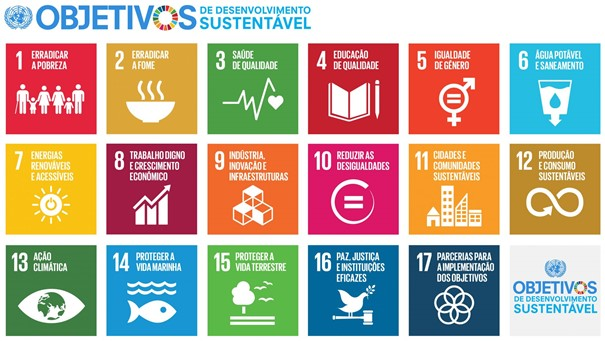
\includegraphics{Imagens/DesenvolvimentoSustentavel.jpg}
    \caption{Objetivos desenvolvimento sustentável ONU}
    \label{fig:ODS}
\end{figure}


\section{Objetivos e perguntas de investigação \label{se:objetivos}}

Foram aprovadas a nível europeu (2020), medidas de alteração aos serviços de sistema, que serão seguidas pelos Estados-Membros. Nesta dissertação far-se-á a aplicação dessas medidas, identificando as melhorias face ao desenho actual e, avaliando se as novas medidas serão suficientes para assegurar a operação de um sistema eléctrico ~100\% renovável, eventualmente identificando acções adicionais que garantam a robustez e segurança do sistema eléctrico sem recurso a combustíveis fósseis.

\begin{description}
  \item[a)]\noindent É positivo para as vRES participar no mercado de reserva?
  \item[b)]\noindent Como configurar essa participação para optimizar o lucro do ponto de vista das vRES?
  \item[c)]\noindent Essa participação é positiva para o sistema eléctrico num todo?
\end{description}

Como forma de responder a estas questões vamos tentar utilizar dados de previsão de geradores renováveis para prever a energia necessária para alocação secundária.\\
Os valores de previsão deste mercado estão actualmente longe do que realmente é utilizado, fazendo com que a alocação no dia anterior não seja em conformidade com o necessario, logo não existindo o optimo aproveitamento de recursos. \\
O objectivo neste trabalho é perceber se utilizando técnicas de \textit{Machine Learning} (Apredizagem automática) %TODO: ver nome em PT para ML, procurar nas teses da fcul
conseguimos obter previsoes mais proximas da energia utilizando, possibilitando assim uma melhor gestão das alocações, logo um menor gasto de recursos, energéticos mas especialmente financeiros.\\

\section{Organização do documento \label{se:organização}}

Este documento está divido em capitulos. Sendo que os primeiros apresentam uma introdução às ideias e temas \ref{ch:introducao}, o estado de arte do temas na literatura publicada \ref{ch:revisao}, e por fim uma contextualização dos temas abordados \ref{ch:contexto}. \\
Segue um capitulo de explicação dos dados usado \ref{ch:dados}, onde se apresentam os mesmos juntamente com alguns estudos preliminares para compreender a naturuza e qualidades dos mesmos. \\%TODO: adicinar onde os buscar e que estudos

O capitulo seguinte entra no ambito experimental da dissertação, onde se apresenta as diferentes arquitecturas \ref{ch:arch} utilizadas, incluindo uma explicação dos componentes das mesmas. \\

Os capítulos 6 e 7 são bastatante paralelos, sendo que o sexto \ref{ch:metodos} apresenta a metologia do trabalho, e explica todas as experiências, e o sétimo \ref{ch:resultados_discussao} apresenta apenas os resultados e conclusoes experiência a experiência. \\

Termina com um capitulo conclusivo \ref{ch:conclusao} onde são avaliadas as experiências como um todo, e o seu impacto no ambito dos mercados de reserva. \\

